%% Template for a preprint Letter or Article for submission
%% to the journal Nature.
%% Written by Peter Czoschke, 26 February 2004
%%

\documentclass{nature}

%% make sure you have the nature.cls and naturemag.bst files where
%% LaTeX can find them

\bibliographystyle{naturemag}
\usepackage[]{algorithm2e}

\title{Urban typologies through city block size and regularity.}

%% Notice placement of commas and superscripts and use of &
%% in the author list

\author{Kerry~A.~Nice$^{1*}$,
Gideon D.P.A. Aschwanden$^{1*}$,
Jasper S. Wijnands$^{1}$,
Jason Thompson$^{1,2}$,
Michele Acuto$^{1}$,
Jingcheng Wang$^{1}$,
Haifeng Zhao$^{1}$,
Mark Stevenson$^{1,3}$,
}







\begin{document}

\maketitle

\begin{affiliations}
 \item Transport, Health, and Urban Design Hub, Faculty of Architecture, Building, and Planning, University of Melbourne, Victoria, Australia
 \item Centre for Human Factors and Sociotechnical Systems, University of the Sunshine Coast, Australia
 \item Melbourne School of Engineering; and Melbourne School of Population and Global Health, University of Melbourne, Victoria, Australia
 \\ \textsuperscript{*} These authors contributed equally to this work
\end{affiliations}

\begin{abstract}

%\begin{summary}
\section{Summary}
% 150 words
% Motivation
Cities are a stage of human interactions, the foundation of society, a large source of pollution, and the habitat of the majority of the world's population. Although each field investigates cities from its own vantage point, we lack an objective method to compare cities around the world and therefore believe that each city is unique. This has led to repeated reinvention of solutions for problems that occur globally. Additionally, the lack of comparable measurement methods between and within cities starves us of the possibility to learn from previous examples.

% Solution
We present a methodology that can reliably compare not only cities but individual neighbourhoods in a robust manner using an unsupervised learning algorithms, a Self Organising Map (SOM), and map imagery created using a global dataset. The SOM projects n-dimensional spaces onto a 2-dimensional plane and can absorb additional data points and alternative data sets.
% Results
This allows us to compare cities as well as individual neighbourhoods of cities with each other, identify similarities of precincts from different cities and similar patterns of urban structures across the globe. We find that city centres and suburban structures are objectively similar across the globe.
% Future
This method can now be deployed to find correlations with other indicators, to help planners and designers create a path to a desirable future and help manage and govern large urban entities by avoiding past pitfalls.


%\end{summary}

% City's 'uniqueness' 
As cities grow and evolve, analysis of the basic structural elements of road networks and urban blocks can provide clues as to the processes and governance under which the development occurred. The built environment has been shown to influence a wide range of outcomes, including health, transport, and economic opportunity. Methods to study cities through these basic structural elements are essential to many disciplines conducting urban research and provide a foundation on which they can conducting their research.
% Implication of city structure and form
 % and in particular / especially the road network and block typology,%


% our solution
We propose a novel, quantitative, and objective method to discover city typologies on a neighbourhood scale of street patterns by evaluating city block size and regularity. This follows Louf \& Barthelemy's finding\cite{Louf2014a} that a systematic quantitative method to identify different neighbourhoods is currently lacking. 
%% solution is globally applicabl | updates easily |  Robust | new city characteristics | can accomodate additonal data |
Our method uses 800x800m imagery from Google Maps of custom, abstract, and stylized maps of the world's largest 1692 cities. Using a  computer vision floodfill technique, the size and regularity of city blocks in imagery samples are calculated and histograms constructed for each. A self organising map (SOM), that deploys an unsupervised learning algorithm, sorts these maps into distinct city block typologies. 

% Results
%% Method is robust visible by global results
%% intra inter city similarities
%% Examples from Melbourne (and other cities)
The proposed methodology has evaluated 1.7 million maps from 1692 cities, showing the robustness of the methodology. The resulting SOM, projecting the high dimensional space onto a 2-dimensional plane, is then used to colour code and highlight the map samples according to their SOM x,y coordinates. This highlights similarity between places and has shown to be able to detect city archetypes such as city centres, suburban areas, and even more ephemeral entities such as the city edges (see figure x [Melbourne\_5.png]).
 
This method is not limited to detecting differences within a city, but is able to use a neighbourhood sample in one city and identify similar locations in all other cities. The global and heterogenous collection of 1692 cities indicates the robustness of the methodology in classifying and identifying typologies in the respective map samples through the SOM.

% Maybe we should add a map segment of melbourne CBD and which other areas in the world are similar.


% Future Work
%% Find correlations with other indicators
Since this methodology promises to be applicable across many fields, the aim of future investigation(s) is to find correlations between urban typologies and other indicators. The potential candidates for such investigations are energy intensity, particular matter, and GDP since they are indicators that are globally available. The logical consequence is to test the methodology towards its predictive power and application in design, planning, and management of urban systems.


%For Nature, the abstract is really an introductory paragraph set
%in bold type.  This paragraph must be ``fully referenced'' and
%less than 180 words for Letters.  This is the thing that is
%supposed to be aimed at people from other disciplines and is
%arguably the most important part to getting your paper past the
%editors.  End this paragraph with a sentence like ``Here we
%show...'' or something similar.
\end{abstract}

%Then the body of the main text appears after the intro paragraph.
%Figure environments can be left in place in the document.
%\verb|\includegraphics| commands are ignored since Nature wants
%the figures sent as separate files and the captions are
%automatically moved to the end of the document (they are printed
%out with the \verb|\end{document}| command. However, tables must
%be manually moved to the end of the document, after the addendum.
%
%Citation of Einstein's paper \cite{Louf2014a}.
%
%\begin{figure}
%%%%\includegraphics{something} % this command will be ignored
%\caption{Each figure legend should begin with a brief title for
%the whole figure and continue with a short description of each
%panel and the symbols used. For contributions with methods
%sections, legends should not contain any details of methods, or
%exceed 100 words (fewer than 500 words in total for the whole
%paper). In contributions without methods sections, legends should
%be fewer than 300 words (800 words or fewer in total for the whole
%paper).}
%\end{figure}
%
%\section*{Another Section}
%
%Sections can only be used in Articles.  Contributions should be
%organized in the sequence: title, text, methods, references,
%Supplementary Information line (if any), acknowledgements,
%interest declaration, corresponding author line, tables, figure
%legends.
%
%Spelling must be British English (Oxford English Dictionary)
%
%In addition, a cover letter needs to be written with the
%following:
%\begin{enumerate}
% \item A 100 word or less summary indicating on scientific grounds
%why the paper should be considered for a wide-ranging journal like
%\textsl{Nature} instead of a more narrowly focussed journal.
% \item A 100 word or less summary aimed at a non-scientific audience,
%written at the level of a national newspaper.  It may be used for
%\textsl{Nature}'s press release or other general publicity.
% \item The cover letter should state clearly what is included as the
%submission, including number of figures, supporting manuscripts
%and any Supplementary Information (specifying number of items and
%format).
% \item The cover letter should also state the number of
%words of text in the paper; the number of figures and parts of
%figures (for example, 4 figures, comprising 16 separate panels in
%total); a rough estimate of the desired final size of figures in
%terms of number of pages; and a full current postal address,
%telephone and fax numbers, and current e-mail address.
%\end{enumerate}
%
%See \textsl{Nature}'s website
%(\texttt{http://www.nature.com/nature/submit/gta/index.html}) for
%complete submission guidelines.













\section{Introduction}\label{sec:introduction}

%% Why is understanding the city so important
%% - Health (Lancet)
%% - Transport (Space Syntax)
%% - Economics (Urban Economics)

\subsection{City Typologies}\label{sec:introduction2}
Cities are the most complex entities humans have ever created, but they are examples of 'organised complexity' that allow us to discern some kind of order within the diversity and complexity cities present \cite{Kropf2014}. Approaches that aim to classify the built form are using a hierarchical dichotomy based on the scale of urban element. Different scales of dichotomies (Figure \ref{fig:TypologyDichtomies}) exist from 3 to 6 steps and range in scale from the building material to the territorial organisation of cities \cite{Lynch1981,Conzen1960,Caniggi1979,Castex1980,Mouden1988,Allain2004}.



\begin{figure}
\centering    
\includegraphics[scale=0.80,page=1]{Images/Typology\_Dichtomies.pdf}  
\caption{\bf Different scales of dichotomies. }    
 \label{fig:TypologyDichtomies}  
\end{figure} 



The used elements by the existing approaches are not coherent, some are using going to the level of rooms, others are expanding on the larger scale. One of the few consistent elements used by all existing approaches is the "Street Block", "Block", "Urban Tissue" or "insula", the area that is confined by the surrounding streets may it be build up, open space or a combination of both.
The evaluation and classification based on the individual dichotomy is 











\begin{methods}
%Put methods in here.  If you are going to subsection it, use
%\verb|\subsection| commands.  Methods section should be less than
%800 words and if it is less than 200 words, it can be incorporated
%into the main text.
%
%\subsection{Method subsection.}
%
%Here is a description of a specific method used.  Note that the
%subsection heading ends with a full stop (period) and that the
%command is \verb|\subsection{}| not \verb|\subsection*{}|.




%\section{Methods}\label{sec:Methods}

\subsection{Map imagery sampling.}\label{sec:methods2}
The concept employed in this study was to sample maps of individual city sections, calculate block size and regularity of each section, and then use a self organizing map (SOM) to organise the images into different urban types. 1692 cities with populations $>$ 300,000 people \cite{UN2014} were selected for analysis. Map imagery from Google Maps \cite{GoogleStatic2017} was used to provide globally consistent data. 

A two-stage sampling approach was applied to each city. As no standardised urban boundaries are available for all the cities evaluated in this study, a methodology had to be developed to define these. Firstly, a sampling area extending 1.5 km from the identified city centroid \cite{UN2014} was set as a baseline. Then the sampling radius $r$ (km) was scaled, increasing by a power of 0.85 to the proportional increase in population size based on \cite{Barthelemy2016} in 

\begin{equation}
r = \sqrt{ \frac{28.27}{\pi} \left( \frac{p}{300,000}  \right) ^{0.85} }
\end{equation}


Standardising the sampling area in this manner avoided socio-political discrepancies relating to a city's `true' (political) boundary and captured differences in population density and shape between small (e.g., Wellington, New Zealand; Izmit, Turkey) and global mega-cities (e.g., Tokyo, Japan;  Delhi, India). Location sampling areas were adjusted for the earth's curvature \cite{Sinnott1984}. Large water-bodies (e.g., oceans but not coastlines) were removed from the sampling area, as they were not indicative of urban form. 

These procedures result in a population and water body-adjusted circular area centred on the city's central coordinates, capturing the widest extent of each city while minimising the amount of non-urban locations. For example, Figure \ref{fig:parissample} shows the resulting sampling locations used in collecting imagery for Paris. 

\begin{figure}
    \centering    
\includegraphics[scale=0.5]{Images/Paris-StreetView-SampleLocations\_crop.png}  
\caption{\bf Sampling locations for map imagery (from Paris, France) \cite{GoogleStatic2017}.}    
 \label{fig:parissample}  
\end{figure} 



\subsection{Map imagery source.}\label{methodsimagery}

320x320 sized map images were sampled using a zoom level of 16 (covering 800x800m at the equator and 450x450m at higher latitudes) using a custom style defined with the Google Static Maps API\cite{GoogleStatic2017} (see Figure~\ref{fig:maps} for examples of Paris, France). The maps provide a high-level abstraction of road (black) and public transport (orange) networks, green space (green), and water bodies (blue). Any remaining space is coded white. Due to mapping inconsistencies in South Korea, all 25 South Korean cities were removed from the dataset, reducing the number of cities to 1665. 1000 maps were sampled per city. In addition, to enable in depth case studies, maps were sampled for Melbourne and Sydney, Australia at a 400m grid resolution across the greater metropolitan areas, resulting in an additional 23,027 locations for Melbourne and 24,596 for Sydney. The total dataset consists of 1,714,591 images.



\begin{figure}
    \centering    
\includegraphics[scale=0.7]{Images/Map1.png}  
\includegraphics[scale=0.7]{Images/Map2.png}
\includegraphics[scale=0.7]{Images/Map3.png}
\includegraphics[scale=0.7]{Images/Map4.png}
\caption{\bf Four sample Google Maps training data images (from Paris, France) \cite{GoogleStatic2017}.}    
 \label{fig:maps}  
\end{figure} 


\subsection{Calculating block size and regularity.}\label{methodscalc}

Block size and regularity were calculated for each sampled image with the following algorithm, using the Java 8 AWT toolkit \cite{Oracle2018}:

\begin{algorithm}[H]
\SetAlgoLined
\KwResult{List of region sizes and region regularity for an image stored in Sqlite3 database }
 Start at top left point of image;\\
 \While{Locate next white pixel by iterating across rows and columns}{
  Floodfill area using boundaries of all non-white colors (i.e. black roads, green space, blue water);\\
  Count pixel size of region;\\
  Find x1 in region with the lowest x value;\\
  Find y1 in region with the lowest y value;\\
  Find x2 in region with the highest x value;\\
  Find y2 in region with the highest y value;\\
  Construct rectangle using the four vertices (x1,y1), (x1, y2), (x2,y1), (x2,y2);\\
  Floodfill and count the number of pixels outside of the rectangle as measure of irregularity;\\
  Add size and regularity counts to list for the image;\\
 }
 Store list in database;\\
 \caption{Calculation of block sizes and regularity}
\end{algorithm}


Sample results are shown in Figure \ref{fig:floodfilled}.

\begin{figure}
    \centering    
\includegraphics[scale=0.3]{Images/city82-745994-result.png}  
\includegraphics[scale=0.3]{Images/city1667-82612-result.png}
\caption{\bf Results of flood filled city blocks.}    
 \label{fig:floodfilled}  
\end{figure} 

\subsection{City size and regularity histograms.}\label{methodshist}

Using the calculated counts, two vectors were constructed for each image, one each for block size and block regularity. The vectors were sorted into 15 histogram bins, the number of bins determined by Sturges' formula \cite{Sturges1926}. To reduce the clumping of data in the first bin, variable bins were used to spread this data across all bins. The first bin starts with a size boundary of 1 and each following bin has a boundary of the current bin boundary times a multiplier. A multiplier of 2.3 was used to fit the maximum count size (320x320 pixels = 102400) into the 15 bins.

The resulting histograms for sample map regions are shown in Figure \ref{fig:mapsandHist}. Histograms input into the SOM were constructed by combining the 15 bins of region size frequencies (on the left side) with the 15 bins of region regularity (on the right) into a single histogram vector.


\begin{figure}
    \centering    
\includegraphics[scale=0.34]{Images/{city169\_5798\_39.739486,-105.019810}.png}  
\includegraphics[scale=0.34]{Images/{city169\_455115\_39.737462,-105.021318}.png} 
\includegraphics[scale=0.34]{Images/{city169\_59949\_39.732605,-105.016022}.png} 
\includegraphics[scale=0.34]{Images/{city1521\_754459\_36.078403,-79.813528}.png} 
\includegraphics[scale=0.06]{Images/Combinedcity169-5798.png}
\includegraphics[scale=0.06]{Images/Combinedcity169-455115.png}
\includegraphics[scale=0.06]{Images/Combinedcity169-59949.png}
\includegraphics[scale=0.06]{Images/Combinedcity1521-754459.png}
\caption{\bf Four samples of map regions (top) and resulting histograms (bottom). Region size and regularity are joined into a combined histogram, with size frequencies on the left side of the graph and regularity on the right.}    
 \label{fig:mapsandHist}  
\end{figure} 


\subsection{Organising maps in the self organising map.}\label{methodscluster}
The self organizing map (SOM) methodology \cite{Kohonen1982} is a data driven technique that transforms a $n$ dimensional data source into a lower dimensional space, commonly a 2-dimensional map, while keeping the relative n-dimensional proximity of two datapoints intact. The distance in the lower dimensional representation is therefore a similarity index of the higher dimensional space. Each point in the 2-dimensional map has location (x,y) and is associated with a vector of values from the n-dimensional space $(V_{x,y} = [v_{1},v_{2},...,v_{n}])$.

SOM is a generic, objective and robust methodology that has been deployed in many domains and is used for the visualization of n-dimensional data and data exploration \cite{Koleheimen2004}. This methodology was chosen for its ability to create 2-dimensional maps of smoothly changing patterns from the original high dimensional space. Additionally the SOM map spans the extremes observed in the original data and allows for investigation on how the data is distributed, potential paths between two observations or function approximation with non-linear relations \cite{Barreto2006}. 

The 1.7 million maps histograms with 30 dimensions were the initial data space used to train the 2-dimensional SOM (written in Java 8 \cite{Oracle2018}). After the randomised initialisation of the 100x100 nodes of the SOM, a random selection of 3.2 million datapoints from the initial data space were used to transform the 2-dimensional SOM to match it. This iterative process locats nodes that are similar to the training vector and morphs the values of the SOM nodes towards the training values. This training is subjugated to a decay function for both magnitude ($learningDecay$) and  distance ($radiusDecay$) in the SOM calculated with


\begin{equation} 
radiusDecay = radius * e^{-1 * iteration / timeConstant}
\end{equation}
where $radius$ is $100/2=50$, $iteration$ is the current training iteration, and $timeConstant$ is $totalIterations / \log _{10} (radius)$. Learn decay is calculated as
\begin{equation} 
learnDecay = learnRate * e^{-1 * iteration / timeConstant}
\end{equation}
where $learnRate = 0.05$.

After the SOM was trained, each map histogram was classified to find the closest matching neuron in the SOM. The underlying imagery of the resulting trained SOM was visualised by tiling representative map images from each node x,y point in the SOM in Figure \ref{fig:somresults}. Areas with black have no associated map segments with that particular node x,y location. Most nodes are associated with multiple map segments that have similar characteristics, %(ref{fig:SOM_density.)
Two notable outliers exist that accumulate more than 10,000 map segments (0:21) with 50104 and (6:72) 10723. Both contain map segments that are either only white (0:21) or contain no white (6:72).

\begin{figure}
\centering    
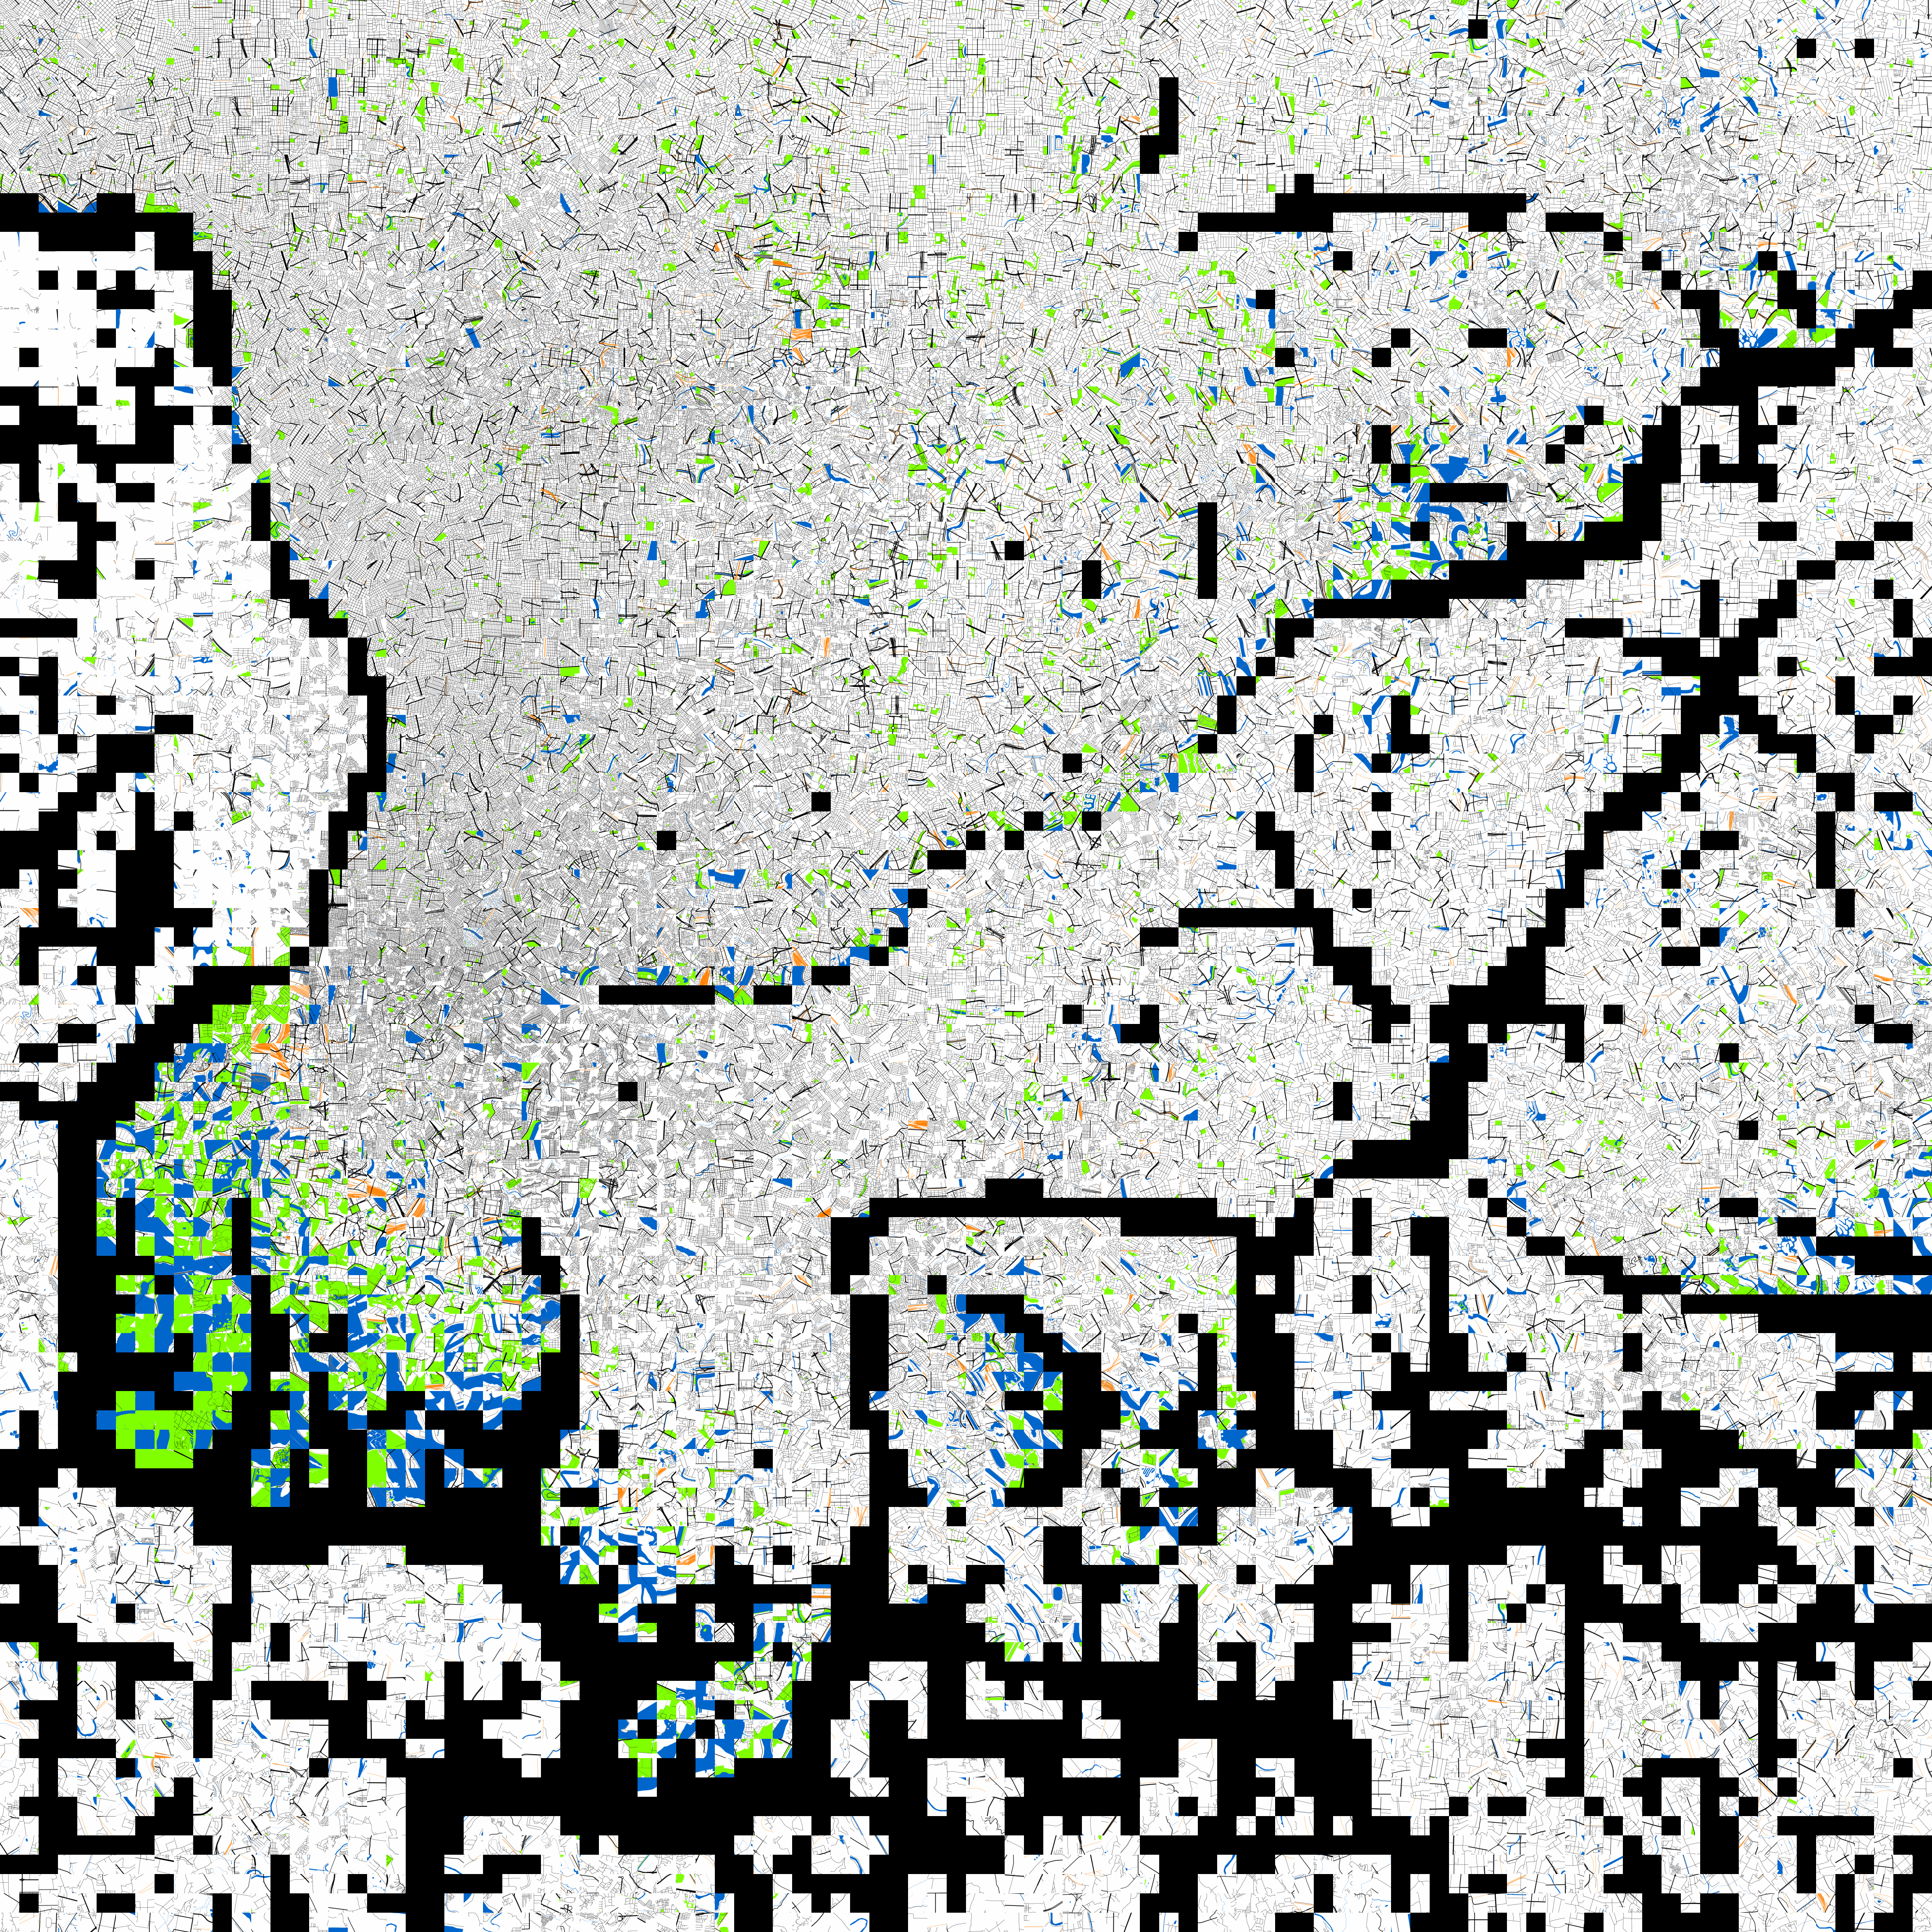
\includegraphics[scale=0.10]{Images/SomImages.png}  
\caption{\bf  A visualisation of the 2 dimensional SOM trained with 1.7 million map images.  Each x,y point shows Left: a representative image associated with each node while nodes without associated images are shown in black and Right: number of images associated with each node}    
 \label{fig:somresults}  
\end{figure} 



The node's x,y locations were encoded into RGB colour code using a Java 8 port of Color2D  \cite{Jackle2017}, based on \cite{Steiger2015}. These colours were used in plotting the x,y typologies in Qgis \cite{QGIS2009}.


\begin{figure}
\centering    
\includegraphics[scale=0.70,page=1]{Images/Melbourne\_5\_Final.pdf}  
\caption{\bf  Map of Melbourne, Australia with 24027 individual map segments classified and colour coded. Note, the CBD shows additional points due to inclusion of the 1000 circular sampling procedure in addition to the 23,027 locations sampled at 400m resolution. }    
 \label{fig:mel23000}  
\end{figure} 






\end{methods}

%% Put the bibliography here, most people will use BiBTeX in
%% which case the environment below should be replaced with
%% the \bibliography{} command.

% \begin{thebibliography}{1}
% \bibitem{dummy} Articles are restricted to 50 references, Letters
% to 30.
% \bibitem{dummyb} No compound references -- only one source per
% reference.
% \end{thebibliography}

\bibliographystyle{naturemag}
\bibliography{bib}


%% Here is the endmatter stuff: Supplementary Info, etc.
%% Use \item's to separate, default label is "Acknowledgements"

\begin{addendum}
 \item Put acknowledgements here.
 \item[Competing Interests] The authors declare that they have no
competing financial interests.
 \item[Correspondence] Correspondence and requests for materials
should be addressed to A.B.C.~(email: myaddress@nowhere.edu).
\end{addendum}

%%
%% TABLES
%%
%% If there are any tables, put them here.
%%

%\begin{table}
%\centering
%\caption{This is a table with scientific results.}
%\medskip
%\begin{tabular}{ccccc}
%\hline
%1 & 2 & 3 & 4 & 5\\
%\hline
%aaa & bbb & ccc & ddd & eee\\
%aaaa & bbbb & cccc & dddd & eeee\\
%aaaaa & bbbbb & ccccc & ddddd & eeeee\\
%aaaaaa & bbbbbb & cccccc & dddddd & eeeeee\\
%1.000 & 2.000 & 3.000 & 4.000 & 5.000\\
%\hline
%\end{tabular}
%\end{table}

\end{document}
